\documentclass{beamer}

\graphicspath{{img/}}

\usepackage{appendixnumberbeamer}

\usepackage{datetime}
\newdate{defensedate}{25}{10}{2017}

\usepackage{minted}

\usetheme[sectionpage=progressbar,subsectionpage=progressbar,numbering=fraction,
          progressbar=foot]{metropolis}

\usepackage{amssymb}

\title{Optimizing the integration of DPLL and $\mathcal{T}$-solvers}
% \subtitle{with a focus on lazy methods with interpolants}

\date{\displaydate{defensedate}}
\author{%
  Simon Bihel\hfill\url{simon.bihel@ens-rennes.fr} \\
}
\institute{%
  University of Rennes I \\
  \'Ecole Normale Sup\'erieure de Rennes
}

\begin{document}

\maketitle

\begin{frame}{Table of contents}
  \setbeamertemplate{section in toc}[sections numbered]
  \tableofcontents[hideallsubsections]
\end{frame}


\section{Basics of SMT($\mathcal{T}$) optimizations}

\begin{frame}{DPLL($\mathcal{T}$)}
  \begin{center}
    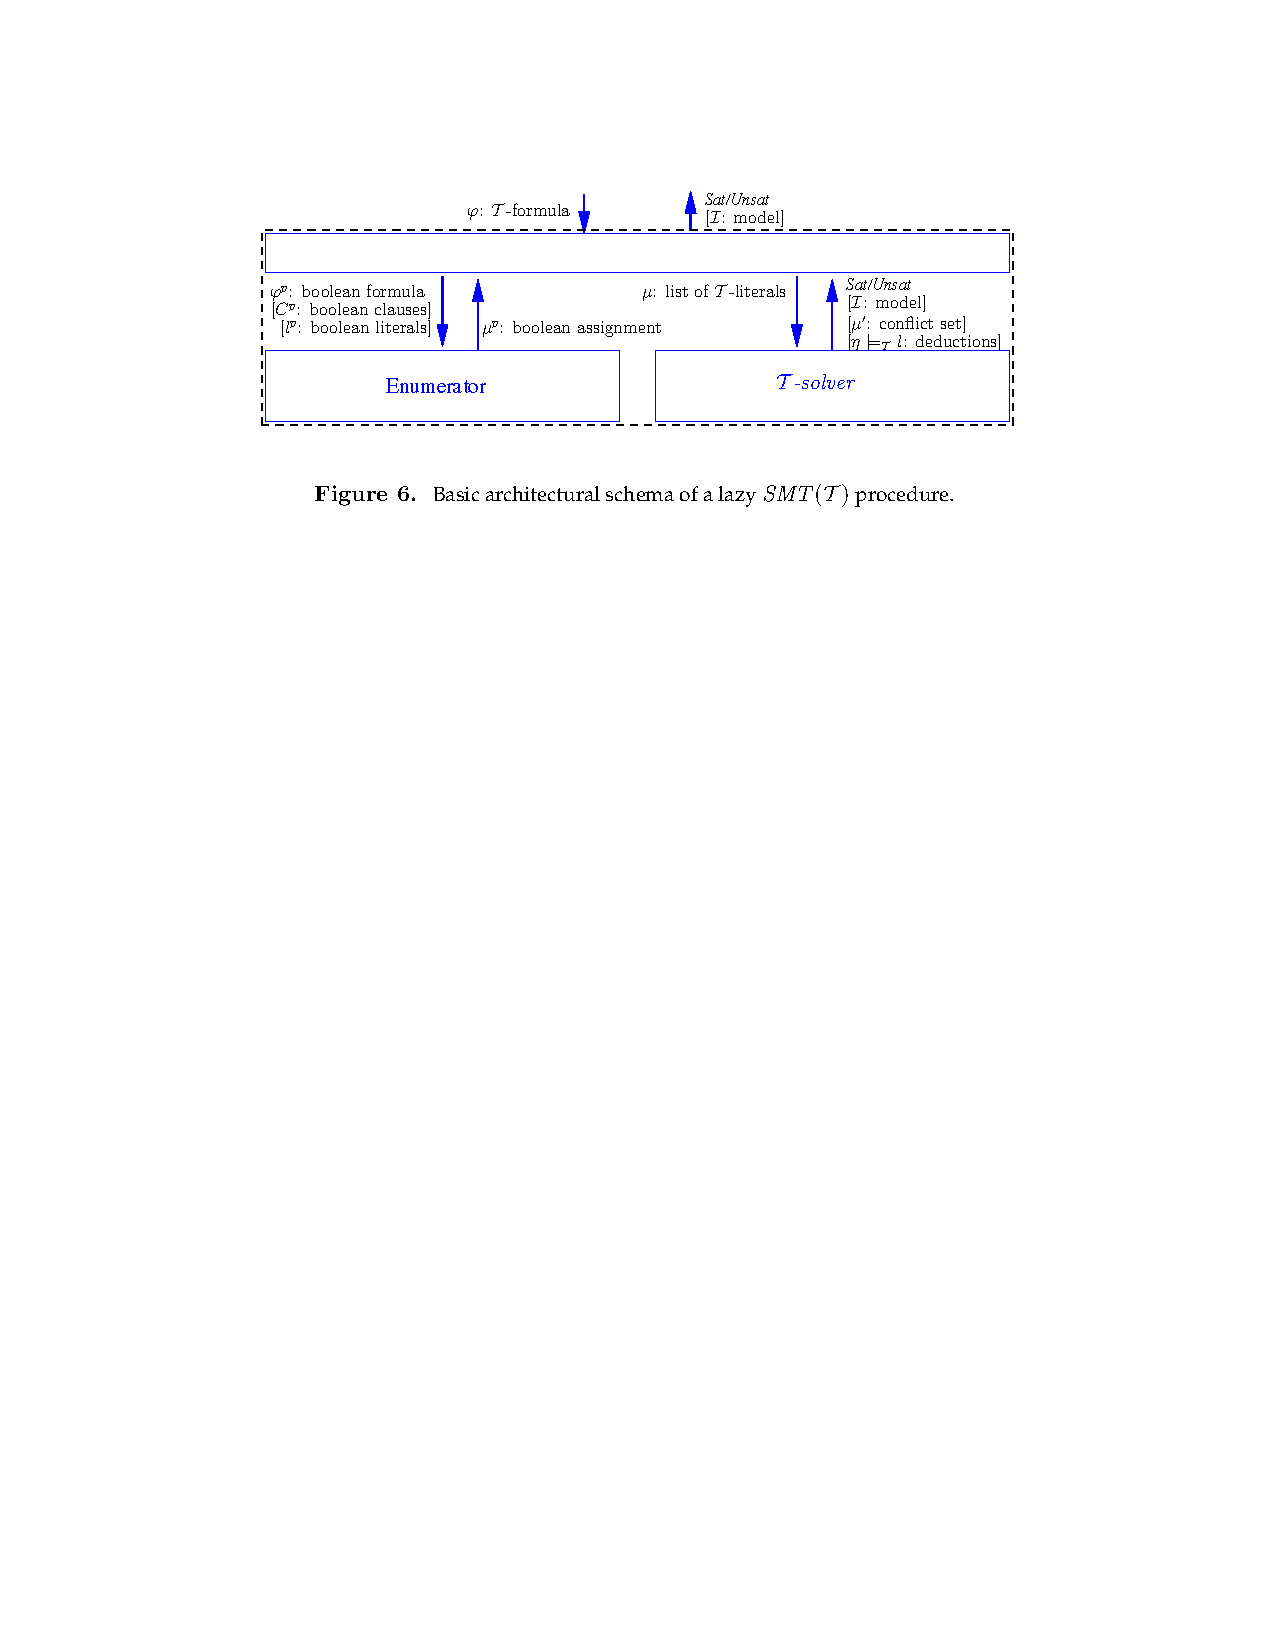
\includegraphics[width=0.9\textwidth]{LazySurvey_fig6}
  \end{center}
  \begin{description}
    \item[Offline] DPLL used as a SAT solver, re-invoked each time an assignment is found $\mathcal{T}$-unsatisfiable.
    \item[Online] DPLL used as an enumerator.
  \end{description}
\end{frame}

\begin{frame}{Interactions between DPLL and $\mathcal{T}$-solver}
  \begin{description}
    \item[Preprocessing] rewrite the input $\mathcal{T}$-formula into a $\mathcal{T}$-equivalent one.
    \item[Look-ahead] Analyze current status to prune the remaining search space.
    \item[Look-back] Recover from a failure and get information to improve future search.
    \item[Assignment simplification] Simplify the assignment for the $\mathcal{T}$-solver.
  \end{description}
\end{frame}

\begin{frame}{Normalizing $\mathcal{T}$-atoms}
  Eliminate $\mathcal{T}$-equivalent $\mathcal{T}$-atoms.
\end{frame}

\begin{frame}{Static learning}
  Prevent ``obviously'' $\mathcal{T}$-inconsistent clauses.

  \begin{exampleblock}{Example}
    Incompatible value assignment

    To prevent $\{x=0, x=1\}$, add $\neg (x=0) \lor \neg (x=1)$
  \end{exampleblock}
\end{frame}

\begin{frame}{Early pruning}
  Intermediate call to $\mathcal{T}$-solver on assignment construction.
  Avoids checking the $\mathcal{T}$-satisfiability of all total truth assignments which extend $\mu$.
\end{frame}

\begin{frame}{$\mathcal{T}$-propagation}
\end{frame}

\begin{frame}{$\mathcal{T}$-backjumping}
\end{frame}

\begin{frame}{$\mathcal{T}$-learning}
\end{frame}

\begin{frame}{Splitting on demand}
  Delegate case-splits to the SAT solver.
\end{frame}

\begin{frame}{Clustering}
  ``Divide-and-conquer'' approach. Partition $\mathcal{T}$-atoms in clusters which do not interfere to each-other's $\mathcal{T}$-satisfiability.
\end{frame}

\begin{frame}{Reduction of assignments}
\end{frame}

\begin{frame}{Pure-literal filtering}
\end{frame}

\begin{frame}{$\mathcal{T}$-deduced-literal filtering}
\end{frame}


\section{Lazy Abstraction with Interpolants}

\begin{frame}{Symbolic Model Checking}
  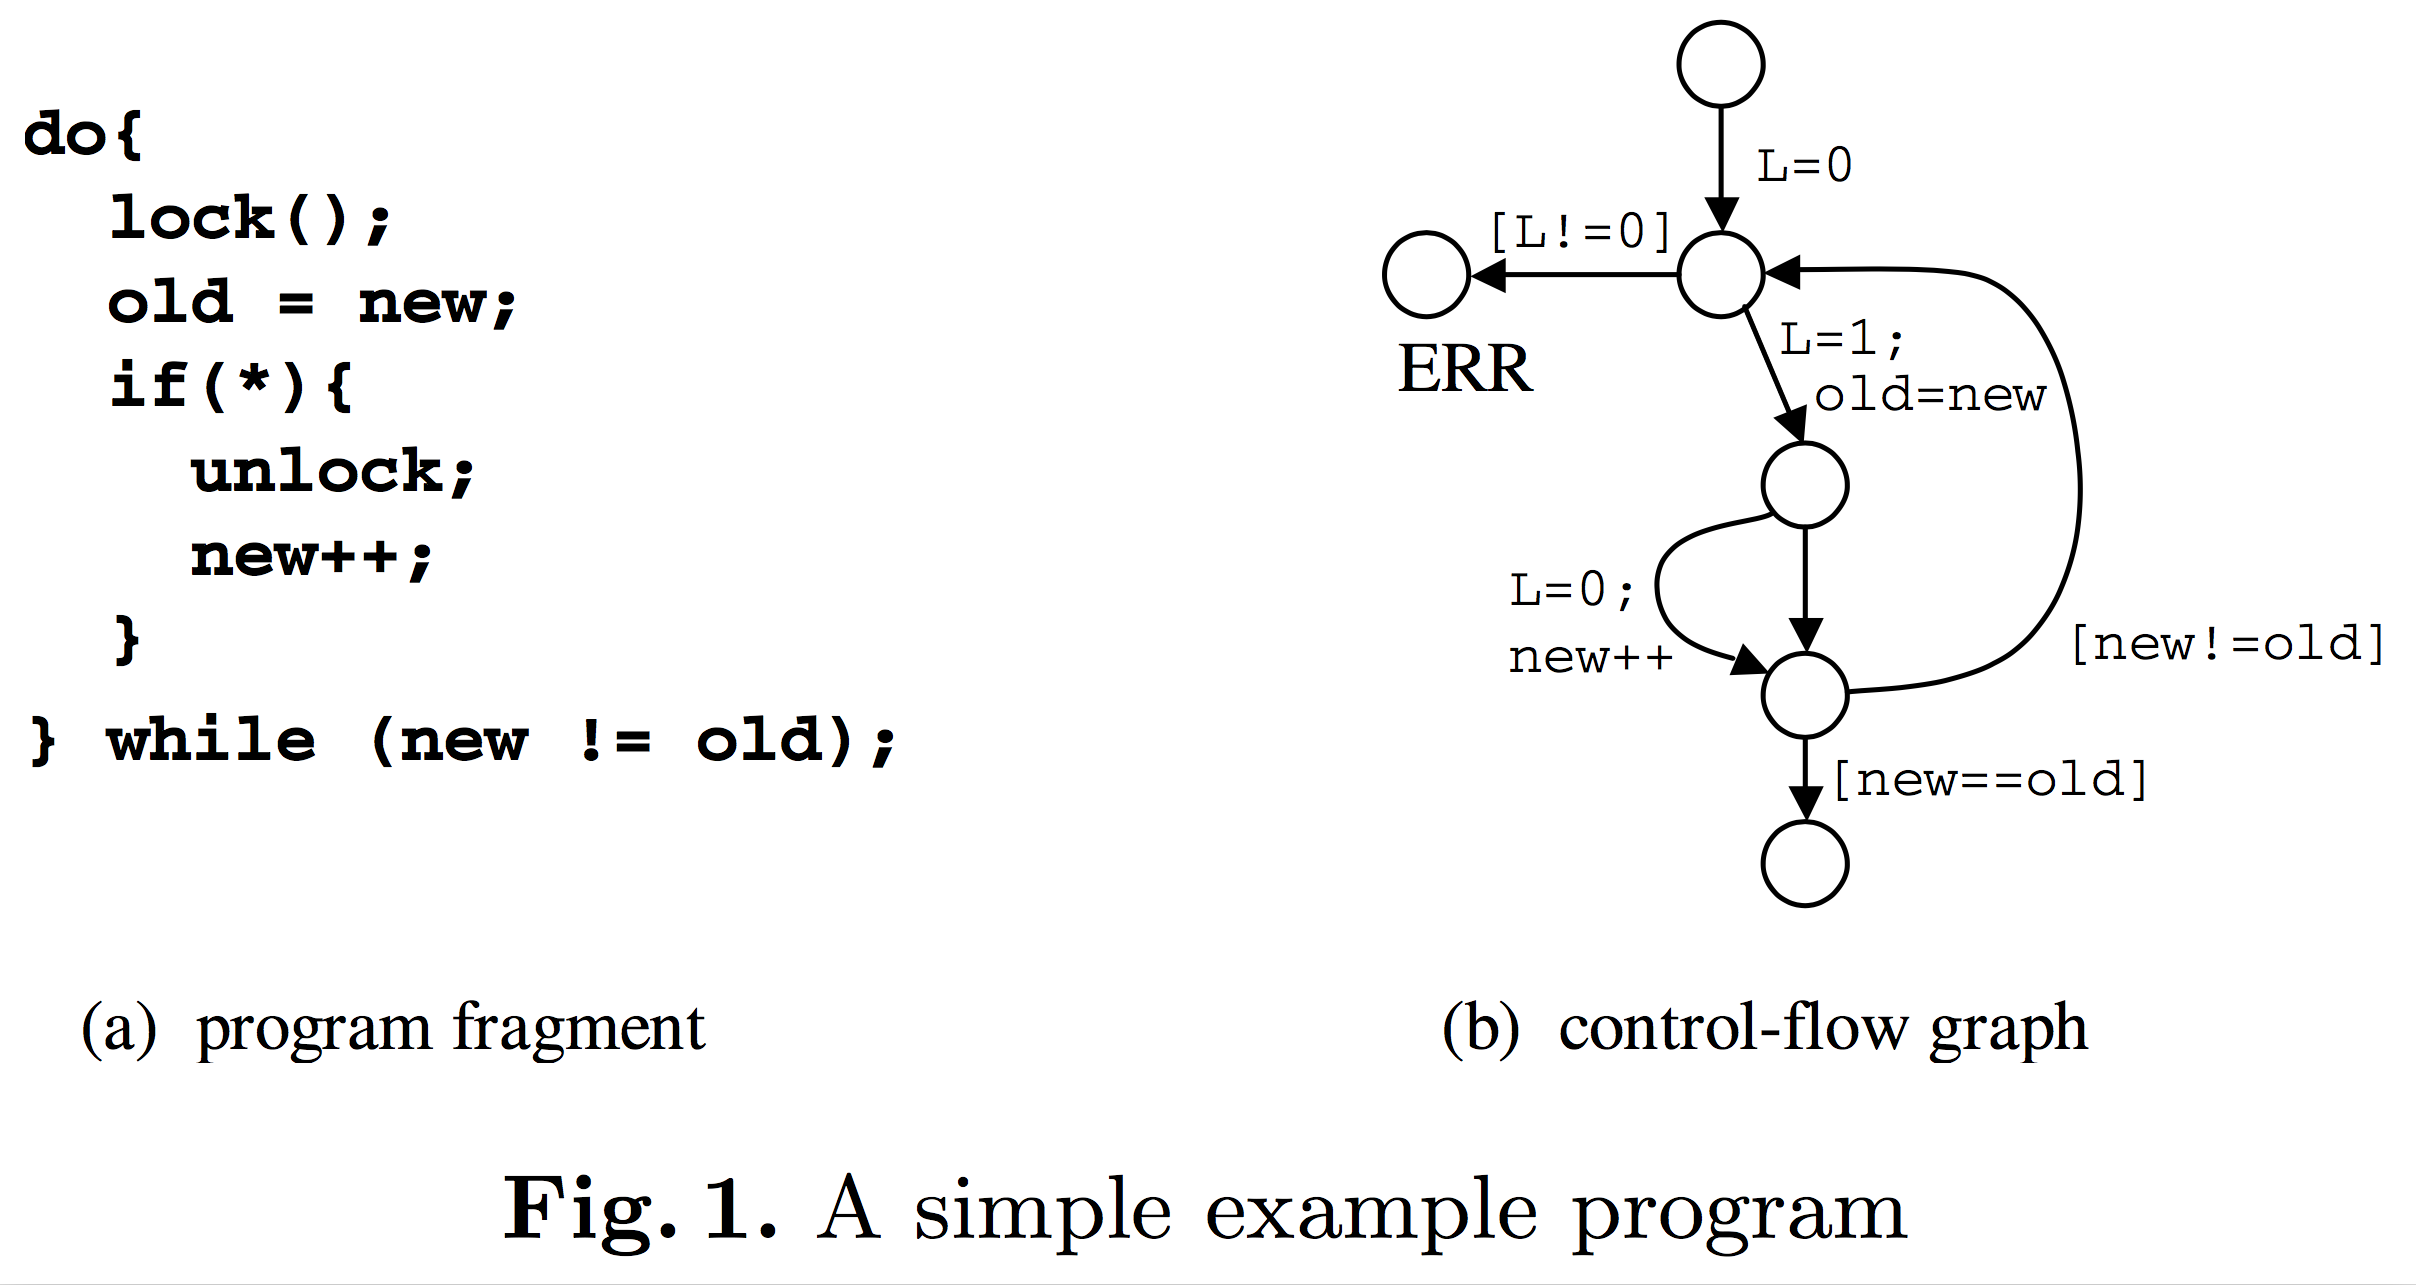
\includegraphics[width=0.9\textwidth]{interpolants_fig1.png}
\end{frame}

\begin{frame}{Interpolants}
  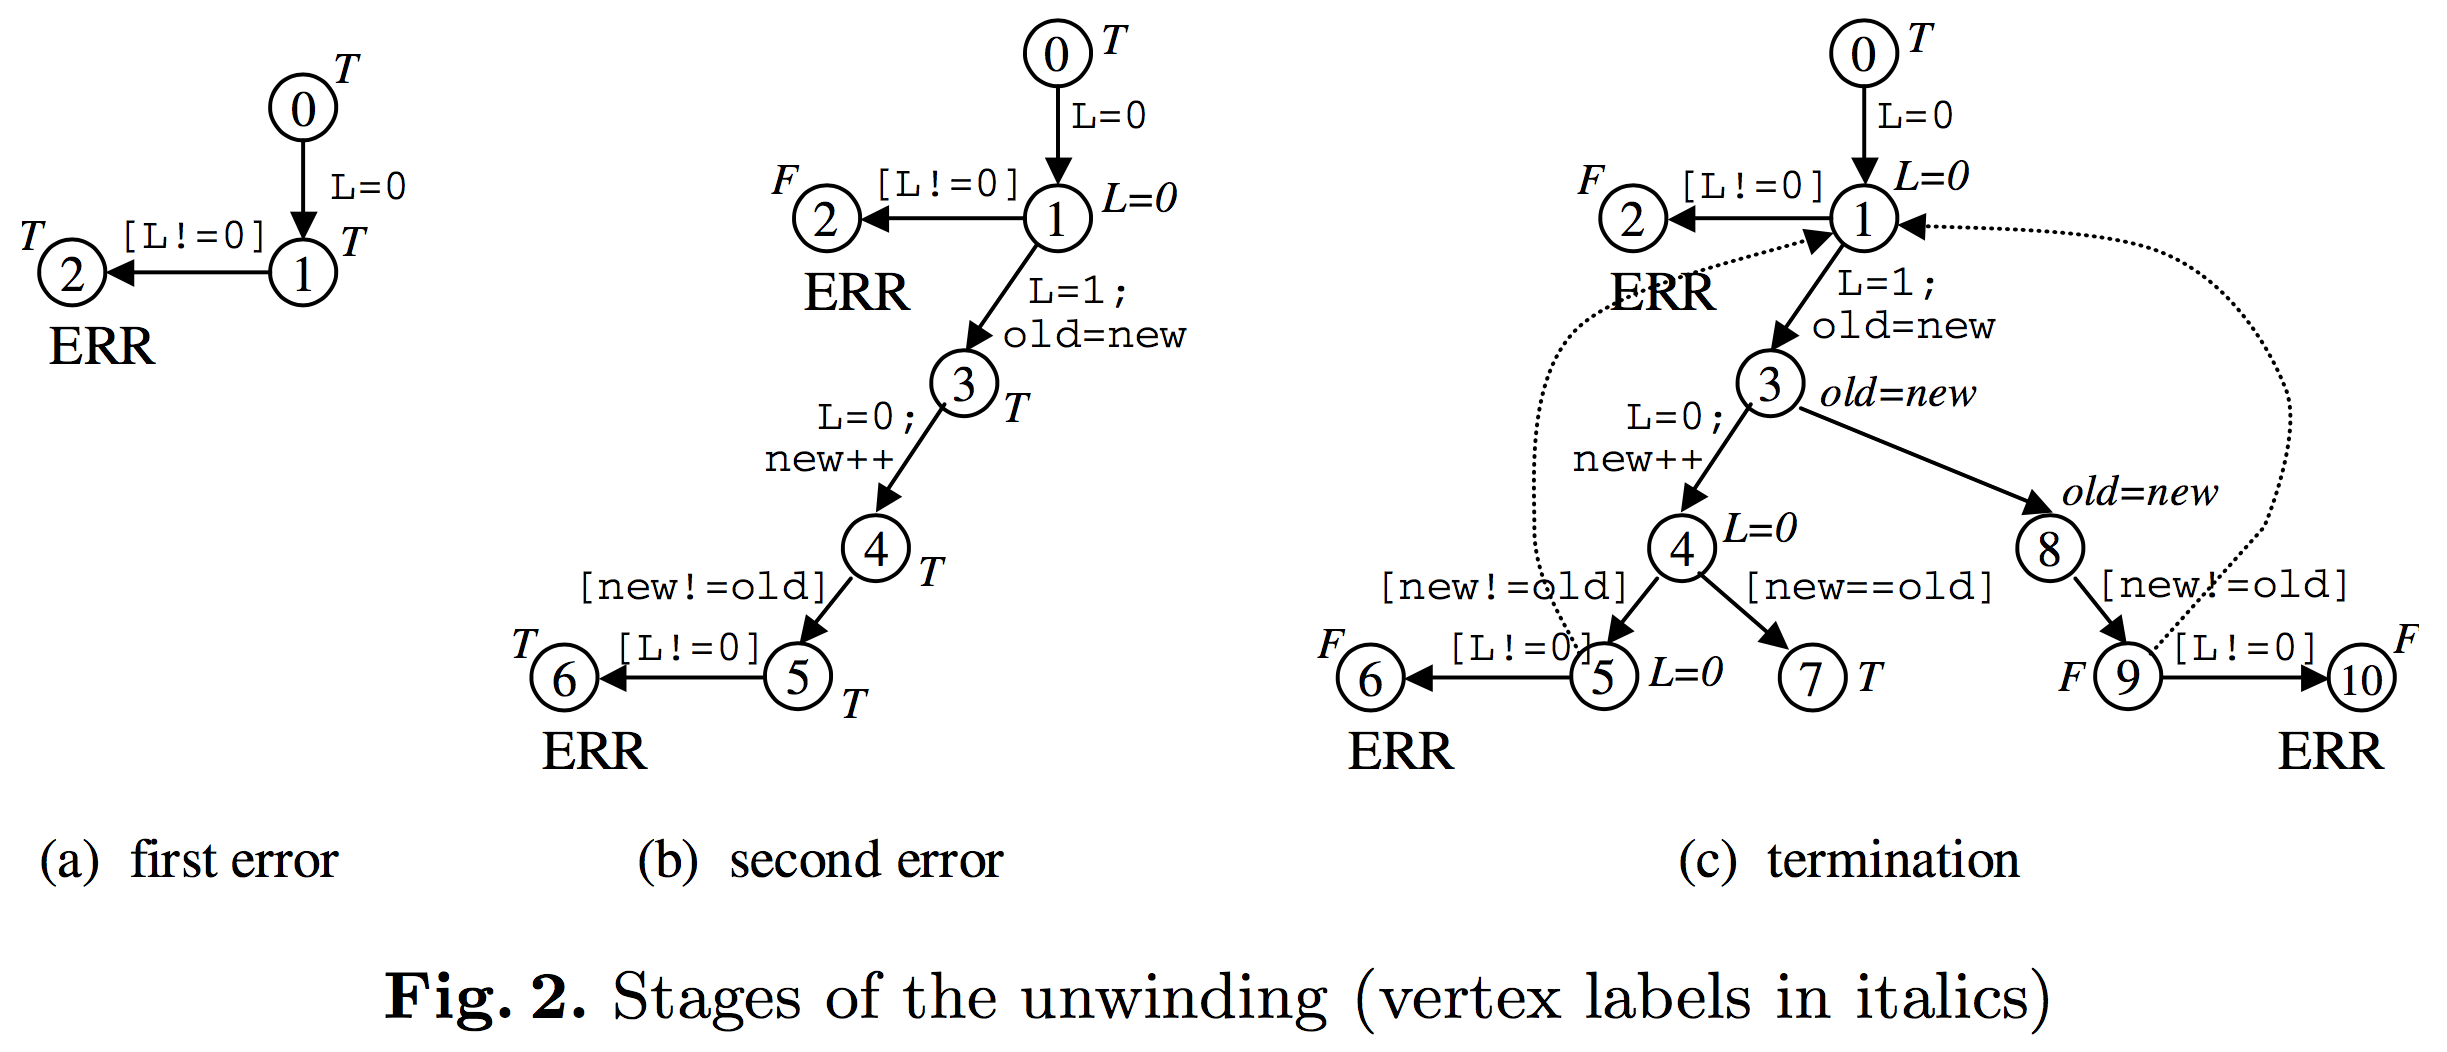
\includegraphics[width=0.9\textwidth]{interpolants_fig2.png}
\end{frame}

\begin{frame}{Other optimization}
  Program slicing, to remove parts of the program having no effect on feasibility of paths.
\end{frame}


% \section*{Conclusion}

% \begin{frame}{Conclusion}
%   Many tools for different situations.
% \end{frame}


\end{document}
